\documentclass[conference]{IEEEtran}
\IEEEoverridecommandlockouts
% The preceding line is only needed to identify funding in the first footnote. If that is unneeded, please comment it out.
\usepackage{cite}
\usepackage{amsmath,amssymb,amsfonts}
\usepackage{algorithmic}
\usepackage{graphicx}
\usepackage{textcomp}
\usepackage{xcolor}
\def\BibTeX{{\rm B\kern-.05em{\sc i\kern-.025em b}\kern-.08em
    T\kern-.1667em\lower.7ex\hbox{E}\kern-.125emX}}
\begin{document}

\title{Analysis of Crimes against Male-Female Employment and Tourism in SriLanka\\
{\footnotesize \textsuperscript}
\thanks{}
}


\author{\IEEEauthorblockN{1\textsuperscript{st} Waruna Priyankara}
\IEEEauthorblockA{\textit{dept. Computer Science and Engineering} \\
\textit{University of Moratuwa}\\
Moratuwa, SriLanka \\
199371p@uom.lk}\\ %
\IEEEauthorblockN{3\textsuperscript{rd} Pumudinee Kumarasiri}
\IEEEauthorblockA{\textit{dept. Computer Science and Engineering} \\
\textit{University of Moratuwa}\\
Moratuwa, SriLanka \\
199338x@uom.lk}
\and
\IEEEauthorblockN{2\textsuperscript{nd} Prageeth Anjula}
\IEEEauthorblockA{\textit{dept. Computer Science and Engineering} \\
\textit{University of Moratuwa}\\
Moratuwa, SriLanka \\
199304p@uom.lk}\\   %
\IEEEauthorblockN{4\textsuperscript{th} Hesitha Wijayasinghe}
\IEEEauthorblockA{\textit{dept. Computer Science and Engineering} \\
\textit{University of Moratuwa}\\
Moratuwa, SriLanka \\
199372u@uom.lk}
}

\maketitle

\begin{abstract}
A significant rise in crime-related incidents is always a major problem for any country. Specially, a developing country like Sri Lanka suffers a lot from crimes. This affects Sri Lanka's economic growth and has a reasonable impact on continuously growing social problems. Theoretical and application-oriented approaches which provide insights into why and where crimes take place are more valuable for decision and policy makers. Geographic information systems and graphical analysis are proven to be essential for studying criminal activities. This paper explores how criminal data relate to male-female employment and tourism industry in Sri Lanka.

\end{abstract}

\begin{IEEEkeywords}
data science, hypothesis, analysis, statistics
\end{IEEEkeywords}

\section{Introduction}
Number of data sets are freely available at Open Data Portal \cite{b2} of SriLanka which is an initiative of SriLanka government to facilitate researches, policy makers and decision makers to come up with ideal solutions for prevailing problems. Crime is a serious problem in SriLanka. Crime related news are published in newspapers each and every day. Authors have chosen data mentioned in Table ``Tab.~\ref{tab1}'' to analyze about criminal activities and their relation between tourism and employment.
Before giving solutions for criminal activities the true reasons behind crimes should be understood. Authors want to see whether there are correlation of crime data with employment and tourism. These data has been recorded as district base. Before analyzing three sets were integrated together. The primary contributions of this paper are:
\begin{itemize}
\item Analyze crime data and male-female employment data for correlation
\item Analyze crime data and tourism data for correlation
\item Use scientific methods in data science for processing, analyzing and visualization
\end{itemize}

\begin{table}[htbp]
\caption{Data set Details}
\begin{center}
\begin{tabular}{|p{3cm}|p{6cm}|}
\hline
\textbf{Data Set}& \textbf{Link}\\[14pt]
\hline
Crime data 2010-2012 & http://www.data.gov.lk/dataset/crime-data-2010-2012 \\[5pt]
Employment by Industrial Sector 2012& http://www.data.gov.lk/dataset/employees-industrial-sector-2012\\[5pt]
Accommodation information for tourists& http://www.data.gov.lk/dataset/accommodation-information-tourists\\[5pt]
Population by district in census years& http://www.data.gov.lk/dataset/population-district-census-years\\[5pt]
\hline
\end{tabular}
\label{tab1}
\end{center}
\end{table}

\begin{figure*}[htbp]
  \centering
    \subfloat{{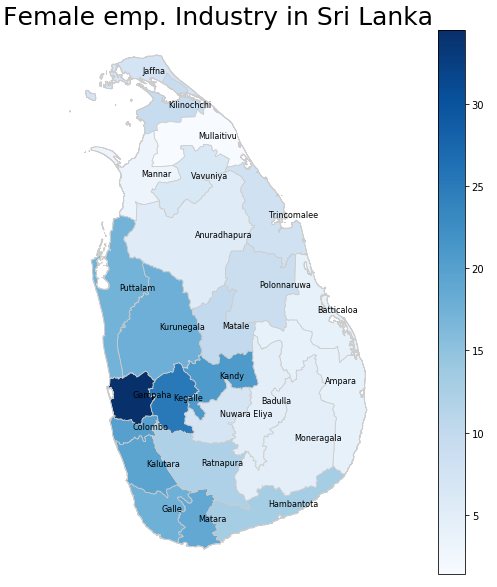
\includegraphics[width=6cm]{female_emp.PNG} }}
    \qquad
    \subfloat{{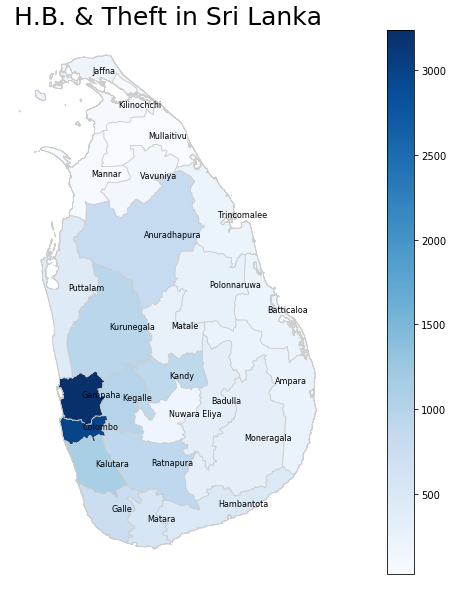
\includegraphics[width=6cm]{crime_HB&theft.PNG} }}
    \qquad
    \subfloat{{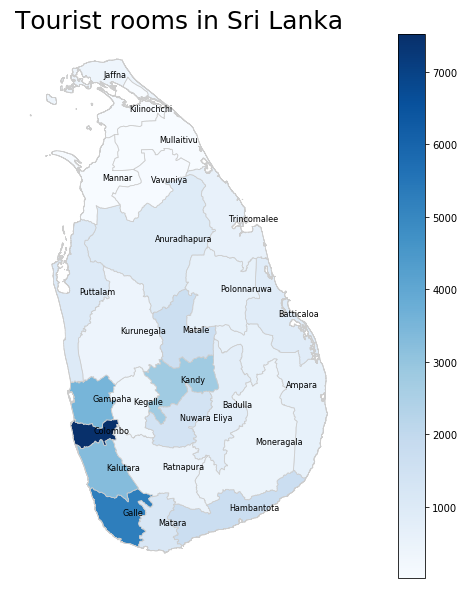
\includegraphics[width=6cm]{tourist_rooms.PNG} }}
     \qquad
    \subfloat{{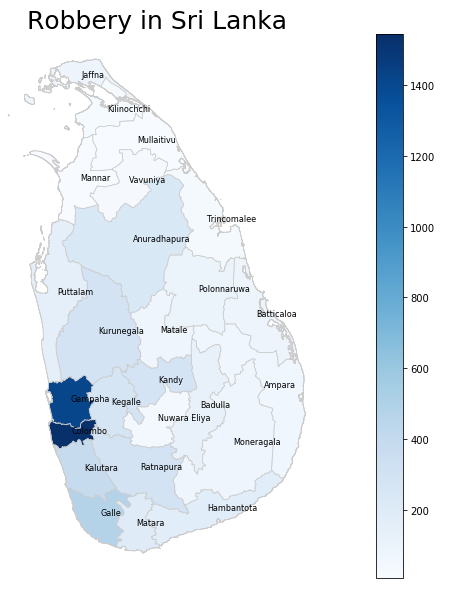
\includegraphics[width=6cm]{crime_robbery.PNG} }}
    \caption{Geo maps for crime}
  \label{fig_geo}
\end{figure*}

\section{Data and Methodology}

\subsection{Data}
Data set and reference to open data portal is mentioned in Table ``Tab.~\ref{tab1}''. Data set dimensions are mentioned below
\begin{itemize}
    \item Crime Data set size =  (25, 23)
    \item Employment Data set size =  (25, 13)
    \item Tourism Data set size =  (2130, 7)
    \item Integrated dataframe shape =  (25, 36)
\end{itemize}
Robbery, abduction, rape crime data distribution throughout the country were plotted.How male-female employment vary across district and room count distribution were also plotted ``Fig.~\ref{fig_geo}''. We can observe that the employed female population is higher in district where abduction/kidnapping is also high. At the same time hotel room count is also higher in district where robbery and other crimes are high.We assume tourism activities are high in districts where totally offered hotel room count is high and it is taken as a measure of the scale of the tourism activity and attraction.  


\subsection{Methodology}
We used the 'pandas' python framework to load and analyze data. Initially, data was loaded to separate data frames. Crime data and employment data were sorted on District and only the total room count per district was taken from the tourism data. The population of each district was also taken into a dataframe and crime counts were normalized by population. All these data frames were integrated to one data frame using district as the common factor since that was available on each data set to prepare a final integrated data frame.

\begin{figure}[htbp]
\centerline{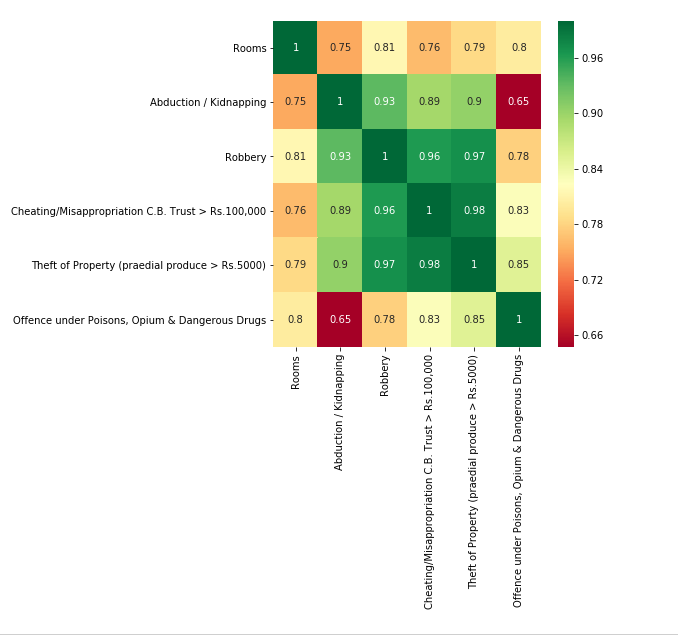
\includegraphics[width=10cm,height=11cm]{fig1.PNG}}
\caption{Heat map of room count with crimes.}
\label{fig1}
\end{figure}
\begin{figure}[htbp]
\centerline{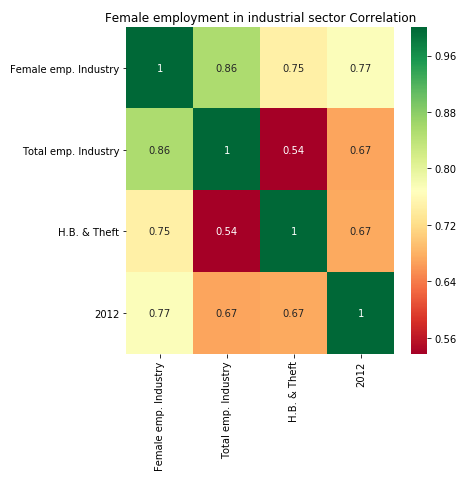
\includegraphics[width=10cm,height=11cm]{fig2.PNG}}
\caption{Heat map of female emp with crimes.}
\label{fig2}
\end{figure}

Room count correlation(Pearson) was calculated and heat map was created for correlation coefficient which is greater than 0.6. ``Fig.~\ref{fig1}'' shows that room count shows a higher correlation with almost all crime data. Robbery and Offence under Dangerous drugs are highly correlated. ``Fig.~\ref{scatter}'' shows scatter plots of each crime and tourism room count. Popular tourism districts such as Colombo, Galle, Gampaha, Kandy, Kalutara districts have recorded higher crimes as well. Each of these districts has more than 2000 tourist rooms, meaning that they are popular tourist destinations.
Two hypotheses are defined with the tourism data.
Hypothesis 1
\begin{itemize}
    \item H0: Number of tourist Rooms and Crimes under Robberies are Uncorrelated
    \item H1: Number of tourist Rooms and Crimes under Robberies are Correlated
\end{itemize}
Hypothesis 2
\begin{itemize}
    \item H0: Number of tourist Rooms and Crimes under "Offence under Poisons, Opium and Dangerous Drugs" are Uncorrelated
    \item H1: Number of tourist Rooms and Crimes under "Offence under Poisons, Opium and Dangerous Drugs" are Correlated
\end{itemize}
Before doing hypothesis testing we did a normality test on our explanatory variable room count and the response variables, robbery and offence under dangerous drugs. We could visualize that though there is a clear correlation between these variables. Although none of the variables were normally distributed. Therefore in order to quantify the correlation, Spearman's Rank correlation was calculated for above two hypotheses. Spearman rank-order correlation is chosen as the statistical procedure that is designed to measure the relationship between two variables where their distribution is unknown. With the results in both cases, we were able to reject the null hypotheses(H0) claiming that there is no correlation between above parameters with 95\% confidence.
A higher correlation was observed between the data for female employment in industrial sector and several categories of crimes such as abduction/kidnapping, Home break and theft, and Hurt by knife ``Fig.~\ref{scatter2}''. Normal distribution test was performed on the above crime data such as abduction/kidnapping, Home break and theft and Hurt by knife and all of them were found to be normally distributed. Therefore below hypotheses were tested for statistical significance with above data.
Hypothesis 1
\begin{itemize}
    \item H0: More Females working in Industrial sector has no relation to high Abduction / Kidnapping
    \item H1: More Females working in Industrial sector has relation to high Abduction / Kidnapping
\end{itemize}
Hypothesis 2
\begin{itemize}
    \item H0: More Females working in Industrial sector has no relation to high Hurt by Knife etc.
    \item H1: More Females working in Industrial sector has relation to high Hurt by Knife etc.
\end{itemize}
Hypothesis 3
\begin{itemize}
    \item H0: More Females working in Industrial sector has no relation to high H.B. and Theft
    \item H1: More Females working in Industrial sector has relation to high H.B. and Theft
\end{itemize}
Before hypothesis analysis data set was split into two samples by female employment count. Low employment and high employment were used to test hypothesis testing. All null hypothesis were rejected by 0.05 significance level.

\begin{figure*}[htbp]
  \centering
    \subfloat{{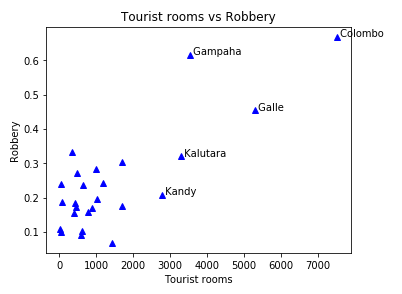
\includegraphics[width=8cm]{scatter1_1.PNG} }}
    \qquad
    \subfloat{{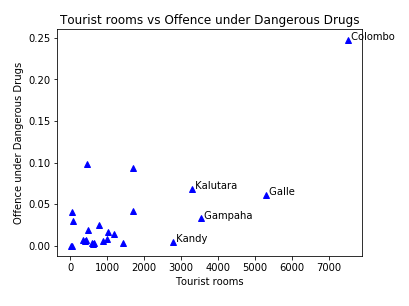
\includegraphics[width=8cm]{scatter1_2.PNG} }}
    \caption{Scatter plots for crime vs tourism rooms.}
  \label{scatter}
\end{figure*}


\section{Results}
After analyzing relationship between crime and tourism/female employment were observed. Popularity of tourism causes a lot of crimes including,
\begin{itemize}
    \item Robbery (0.81)
    \item Dangerous drugs (0.8)
    \item H.B. and Theft
    \item Kidnapping
    \item Offences with weapons
\end{itemize}
Female employment in industrial sector relates to crimes like,
\begin{itemize}
    \item Abduction/ Kidnapping (0.8)
    \item H.B. and Theft (0.77)
    \item Hurt by knife (0.83)
\end{itemize}
High female employment in industrial sector means high high criminal records. Refer scatter plots``Fig.~\ref{scatter2}''.\par
We use a linear model to predict H.B. & theft given a district which has a particular female employment in industrial sector and/or tourism. Ridge regression was used since we have small data set (25 districts). Even though this is not a time-based prediction, still useful to predict theft for a district given female employment in industrial sector. Mean score of 3-fold cross validation
\begin{itemize}
    \item Using female emp. (0.4913)
    \item Using tourism (0.0579)
    \item Using both features (0.5264)
\end{itemize}
Same technique was used for robbery predictions. Predicted robberies given a district with female employment in industrial sector and tourism popularity. Mean score of 3-fold cross validation 
\begin{itemize}
    \item Using tourism (0.4689)
    \item Using female emp. (0.1962)
    \item Using both features (0.6039)
\end{itemize}

\section{Conclusion}
Tourism is often one of the most important driving forces behind the economy of given region, city or country. Tourist attraction is a blessing to the country as it contributes a major portion of the GDP of Sri Lanka. Though, according to our statistical results, there is a significant relationship with tourism and the number of crime categories such as robbery and Offence under Poisons, Opium & Dangerous Drugs showing a higher rate in major tourist destinations. These criminal activities would affect the safety of tourists and the locals of that region. And the increased number of illegal drugs related crimes imposes a grave risk to the lives of the tourists and the residents, which can possibly results in a massive breakthrough to the social and cultural values of the country affecting the future generations as well. In addition, increased number of crimes would result in a reduction of tourist attraction and therefore in a cascading manner it would affect the reputation of the country and the economy as well.\par
Having the above proven results, with a confident of 95\% the high correlation between tourism and crimes such as robbery and Offence under Poisons, Opium & Dangerous Drugs, it is highly advised that the necessary precautionary measures should be taken in order to avoid or minimize those crimes specifically. Sufficient security facilities should be provided to the tourists and additional security officials need to be employed at popular tourism destinations and the locals should be made aware to be more vigilant about the suspicious people or activities in the surrounding and both the tourists and the locals need to be encouraged to escalate such situations to the relevant officials as soon as possible. \par
We were also able to prove with a 95\% confident that there is a high correlation between  female employment in industrial sector and the crime categories such as Hurt by Knife and home break and theft. We ambition this nature is due to the complications that can possibly arise when more females are employed out from their homes at industrial sectors and are undergoing many ill social affairs causing the rise of above crimes such as hurt by knife. The increase in house breaks and theft is possibly because of the idling of houses when even the females are employed out at industrial sectors. In order to mitigate these issues, we encourage the relevant officials to spread this news to the public and to request to take more care to their loved ones working at industrial sectors and be vigilant to the possible risks to their lives and escalate them to the police as early as possible. People should be made that they need to be more careful about the protection of their houses and properties when the females is also employed in industrial sector.
 

\begin{figure*}[htbp]
  \centering
    \subfloat{{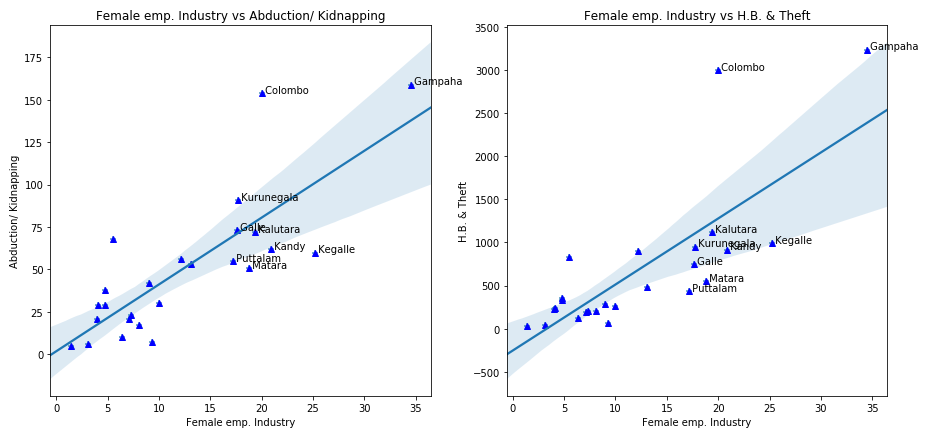
\includegraphics[width=8cm]{scatter2.PNG} }}
    \qquad
    \subfloat{{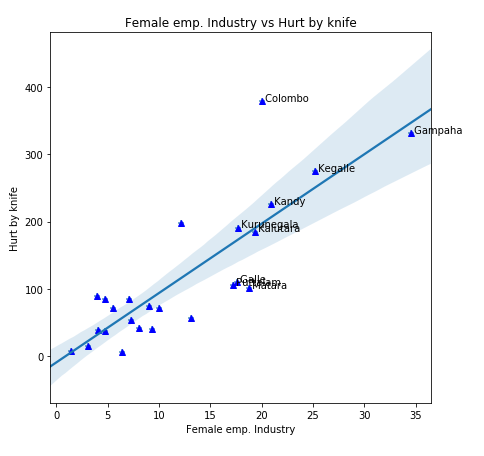
\includegraphics[width=8cm]{scatter3.PNG} }}
    \caption{scatter plot for crime vs female employment}
  \label{scatter2}
\end{figure*}

\begin{thebibliography}{00}
\bibitem{b1} Agnieszka Lisowska, ``crime in tourism destinations: research review,'' Agnieszka Lisowska University of Wroclaw, Institute of Geography and Regional Development,.
\bibitem{b2} open data portal, "http://www.data.gov.lk/".
\bibitem{b3} Discover the beauti of Latex , ``https://www.latex-tutorial.com/'' .
\bibitem{b4} Correlation Calculation "https://machinelearningmastery.com/how-to-calculate-nonparametric-rank-correlation-in-python/"
\end{thebibliography}

\end{document}
